\documentclass[tikz, border=10pt]{standalone}
\usepackage{tikz}
\usetikzlibrary{automata, positioning, arrows.meta}

\begin{document}
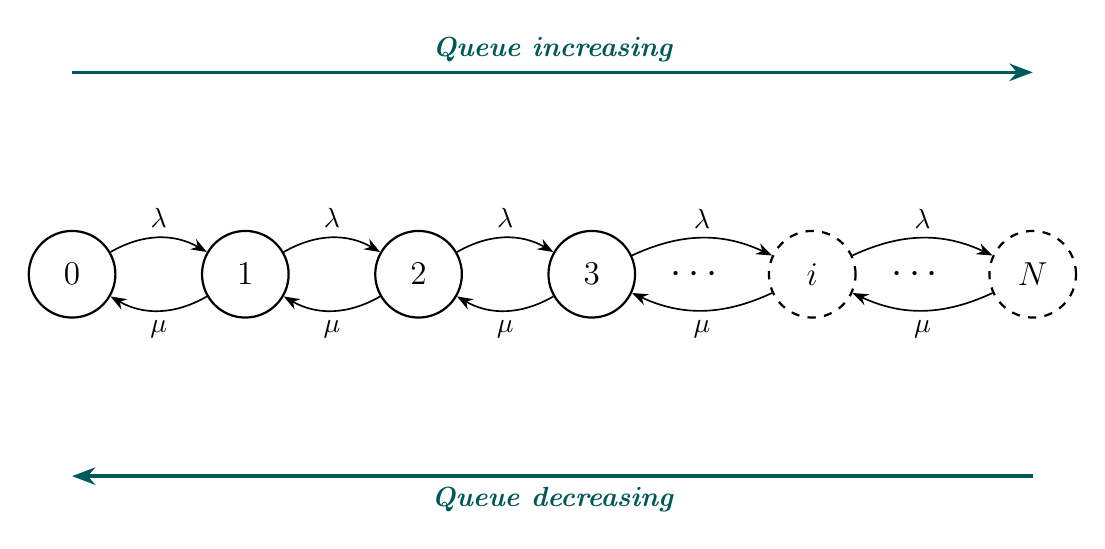
\begin{tikzpicture}[
        % Node style: circular states
        node distance=2.2cm,
        every state/.style={
                circle, draw, thick,
                minimum size=1.1cm,
                font=\large\bfseries
            },
        % Arrow style
        >=Stealth,
        auto,
        semithick
    ]

    %% ---- Solid states: 0, 1, 2, 3 ----
    \node[state] (0) {$0$};
    \node[state, right of=0] (1) {$1$};
    \node[state, right of=1] (2) {$2$};
    \node[state, right of=2] (3) {$3$};

    %% ---- Dashed states: i, N ----
    \node[state, right of=3, dashed, node distance=2.8cm] (i) {$i$};
    \node[state, right of=i, dashed, node distance=2.8cm] (N) {$N$};

    %% ---- Dots between 3 and i ----
    \node[right of=3, node distance=1.3cm, font=\Large] (dots) {$\cdots$};
    \node[right of=i, node distance=1.3cm, font=\Large] (dots2) {$\cdots$};

    %% ---- Forward transitions (lambda, top, bend left) ----
    \draw[->] (0) to[bend left=30]  node[above] {$\lambda$} (1);
    \draw[->] (1) to[bend left=30]  node[above] {$\lambda$} (2);
    \draw[->] (2) to[bend left=30]  node[above] {$\lambda$} (3);
    \draw[->] (3) to[bend left=25]  node[above] {$\lambda$} (i);
    \draw[->] (i) to[bend left=25]  node[above] {$\lambda$} (N);

    %% ---- Backward transitions (mu, bottom, bend left) ----
    \draw[->] (1) to[bend left=30]  node[below] {$\mu$} (0);
    \draw[->] (2) to[bend left=30]  node[below] {$\mu$} (1);
    \draw[->] (3) to[bend left=30]  node[below] {$\mu$} (2);
    \draw[->] (i) to[bend left=25]  node[below] {$\mu$} (3);
    \draw[->] (N) to[bend left=25]  node[below] {$\mu$} (i);

    %% ---- Arrows indicating queue direction ----
    % Top arrow: Queue increasing (right)
    \draw[->, thick, color=teal!70!black, line width=1.2pt]
    ([yshift=2.0cm] 0.north) -- ([yshift=2.0cm] N.north)
    node[midway, above, font=\itshape\bfseries, color=teal!70!black]
    {Queue increasing};

    % Bottom arrow: Queue decreasing (left)
    \draw[->, thick, color=teal!70!black, line width=1.2pt]
    ([yshift=-2.0cm] N.south) -- ([yshift=-2.0cm] 0.south)
    node[midway, below, font=\itshape\bfseries, color=teal!70!black]
    {Queue decreasing};

\end{tikzpicture}
\end{document}